\documentclass[11pt, twocolumn]{article}

\usepackage{float}
\usepackage{math}
\usepackage{graphicx}
\usepackage{indentfirst}
\usepackage{minted}
\usepackage{mathabx}
\usepackage{amsmath}

\title{Final Project: Eye Detection with Random Forests}
\author{Abby Gregory and Andrew Gibiansky}
\date{December 5$^\text{th}$, 2013}

\setlength\parindent{1cm}

\begin{document}
\maketitle

\section*{Overview}

\section*{Image Keypoints and SIFT}
To detect eyes in images, we begin by detecting all interesting locations in the image. These locations,
also known as keypoints, are traditionally detected using corner, edge, or blob detectors. Focusing
on the regions around these keypoints allows us to classify interesting pieces of the image, and
allows us to use our algorithms with any images.

In order to classify keypoints, we need to represent each keypoint as a feature vector that we can
use as input to a machine learning algorithm. For example, we could represent each keypoint as the
intensities of its surrounding pixels. However, if we rotated an image by 90 degrees or scaled it to
half its size, our algorithm would no longer be able to classify the image in the same way.
The Scale-Invariant Feature Transform (SIFT), a commonly-used method in computer vision, provides a
representation of any keypoint as a scale and rotation-invariant 128-dimensional vector. The
components of these vectors roughly correspond to information such as image-color gradients'
magnitudes and orientations.

\section*{Decision Trees}
A decision tree is a classifier which operates via discrete divisions of the data according to their
attributes. Each node of the decision tree represents either a decision (if the node is internal to
the tree) or a class (if the node is a leaf). During classification of a particular example, the
tree is traversed starting from the root. Each node directs the example by examining
particular attribute of that example. In the case of numeric attributes, decision trees use
thresholds to determine the branch to follow; in the case of nominal attributes, each attribute can
map to a single branch of the tree. When the classification reaches a node, the class at that node
is returned as the prediction of the decision tree.

To build a decision tree, we begin by choosing the best attribute and numeric threshold for that
attribute. We define the best attribute as the one which maximizes the information gained, which we
can compute by looking at the entropy of the class distribution before and after we split on that
attribute. We then divide our dataset by splitting on the attribute and then recurse on each branch.
When built with this algorithm, decision trees are prone to overfitting, but we can mitigate this by
combining many decision trees into a single ensemble learner.

\section*{Random Forests$^\text{\textregistered}$}
A random forest is a type of ensemble learner specific to decision trees. In order to create an
effective ensemble learner, random forests are composed of trees that are forced to be significantly
different from one another. This ensures that when the trees make mistakes, they make mistakes on
different elements, so that at least some trees will classify each element correctly.

When training a random forest, we begin by taking one bootstrapped sample for each decision tree we
want to train. Given some dataset, a bootstrapped sample drawn from this dataset is a dataset
composed of elements randomly sampled (with replacement) from the original dataset. In our
algorithms, we used bootstrapped samples of the same size as the original dataset itself. This
bootstrapping process ensures that the trees see different data and thus grow to be different.

For each bootstrapped dataset, we train a decision tree. The decision trees used by random forests
are specialized: at each node, instead of choosing the best attribute of \emph{all} the attributes,
they choose the best of a randomly chosen subset of all the attributes. Once more, this ensures that
the trees end up very different from one another, because they cannot choose the same attributes to
split on in the same places.

\section*{Implementation}
We implemented decision trees, bootstrapping, and random forests in Java. Our decision trees were
entirely unpruned, and could only operate on numeric attributes. We assumed that the values of the
attribute were approximately normally distributed, and therefore we could use the mean of all of the
attribute's values as its split-point. The best attribute from the available subset was, as usual,
determined via the information-gain heuristic. We stopped growing the tree when we had no more
attributes or when the available data was less than 4\% of our dataset in the hope that this would
reduce overfitting.

When generating random forests, bootstrapped datasets of the same size as the original dataset were
used to train each tree. The number of trees and the size of the attribute subset at each node were
left as parameters.

We used Matlab to handle the image-processing portions of our project. We used a library called
VLFeat that implements SIFT and provides a Matlab interface. Once images had been loaded and
converted into SIFT keypoints, we called our Java implementation of Random Forests to perform
classification.

In order to train and test our classifier, we used the BioID face recognition database. The BioID
database provides approximately 1500 grayscale images of frontal face views of 23 three different
people. In addition, it specifies the pixel coordinates of the pupils of the left and right eyes in
the image. We located keypoints in the image and then classified each keypoint as part of an eye or
not part of an eye depending on the distance from the actual centers of the eyes as given by the
dataset.

\section*{Results}
In order to examine the effect of hyperparameters on classification, we plotted the classification
accuracy of our model against varying values of each hyperparameter.

First, we examined the effect of the attribute-subset size on the classification accuracy. This
value determines the size of the random subset of the attributes that each node is allowed to choose
from.

\begin{figure}[h!]
    \centering
    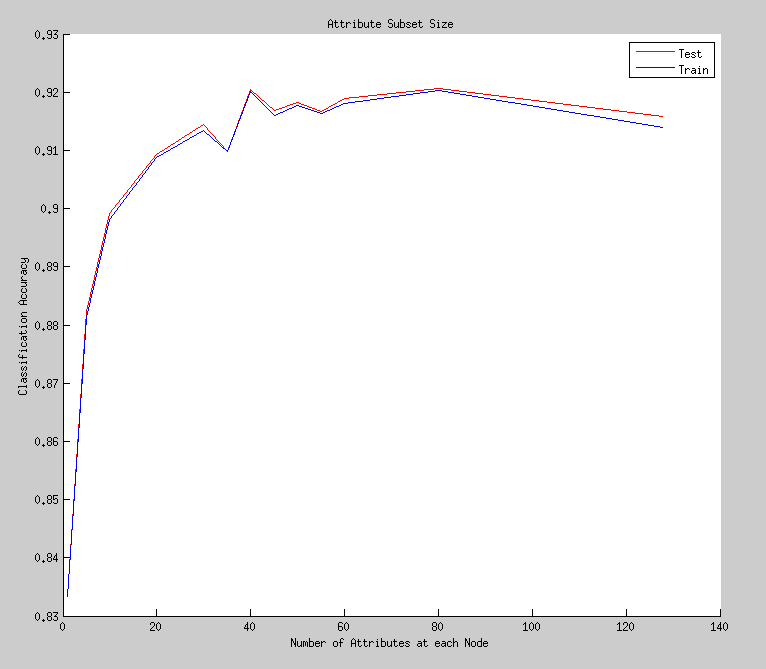
\includegraphics[scale=0.3]{./imgs/attributes.png}
\end{figure}

This graph indicates that increasing the number of attributes has a positive effect on the
classification accuracy up to a certain point. Past that point, adding further attributes decreases
the effectiveness of the random forest. When there are not enough attributes, the decision trees
cannot choose useful attributes to split on because they are rarely available. Once we allow many
attributes, however, the decision trees become very similar, and the effectiveness of the random
forest as a whole is reduced. Based on our data, the optimal number of attributes with the number of
trees fixed at 35 is around 30.



\begin{figure}[h!]
    \centering
    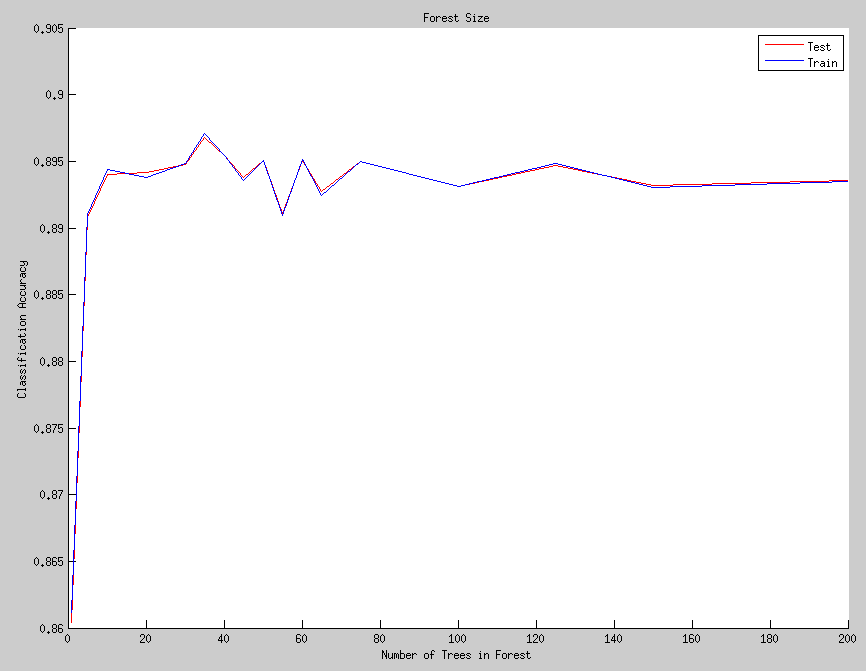
\includegraphics[scale=0.3]{./imgs/trees.png}
    \caption{
        trees.png
    }
\end{figure}

\begin{figure}[h!]
    \centering
    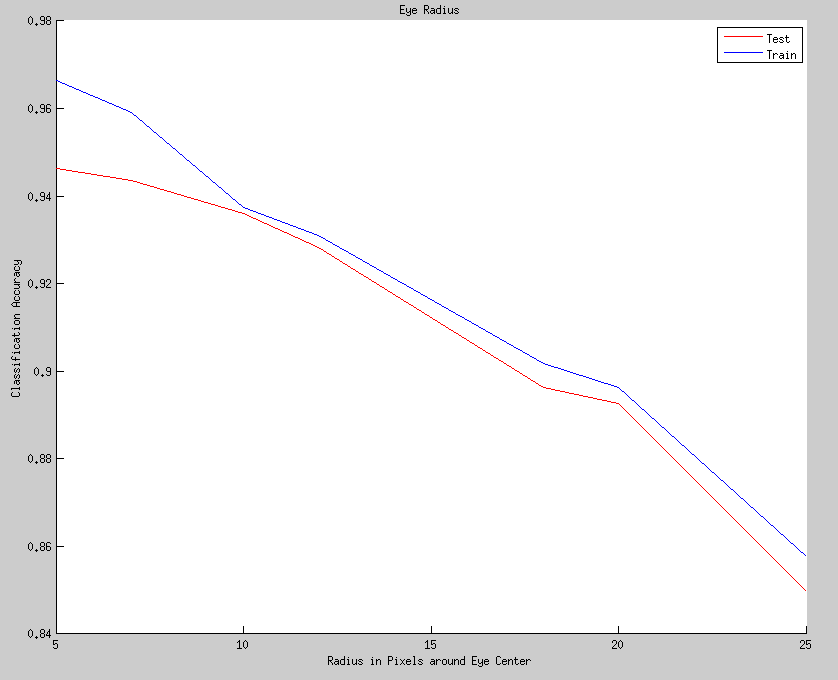
\includegraphics[scale=0.3]{./imgs/radius.png}
    \caption{
        radius.png
    }
\end{figure}

\begin{figure}[h!]
    \centering
    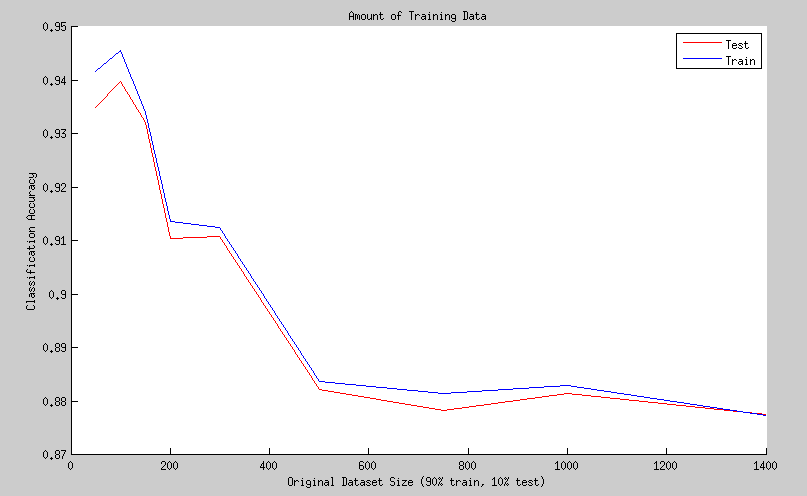
\includegraphics[scale=0.3]{./imgs/dataset.png}
    \caption{
        dataset.png
    }
\end{figure}

To evaluate the performance of our final classifier, we took a twenty second video using a webcam
and plotted keypoints in different colors corresponding to their predicted class.

\begin{figure}[h!]
    \centering
    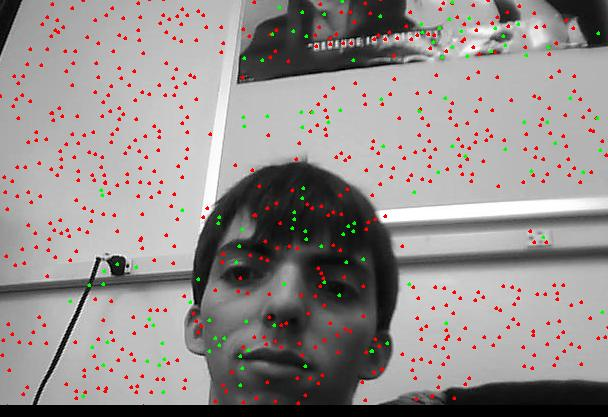
\includegraphics[scale=0.3]{./imgs/silver.png}
    \caption{
        silver.png
    }
\end{figure}

\begin{figure}[h!]
    \centering
    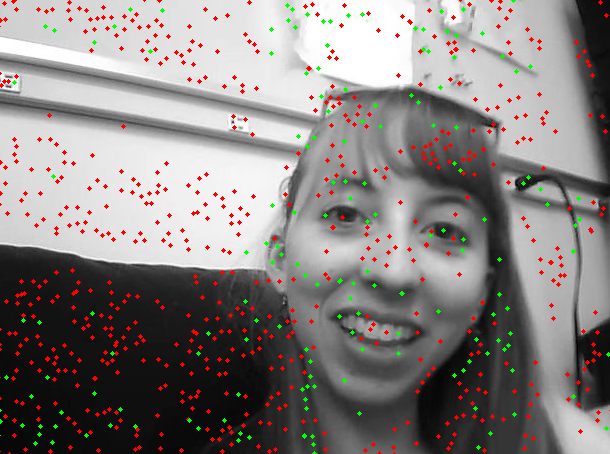
\includegraphics[scale=0.3]{./imgs/abby.png}
    \caption{
        abby.png
    }
\end{figure}

\begin{figure}[h!]
    \centering
    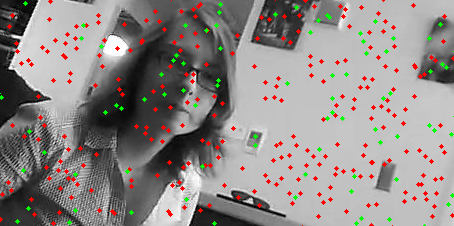
\includegraphics[scale=0.3]{./imgs/rachel.png}
    \caption{
        rachel.png
    }
\end{figure}

\begin{figure}[h!]
    \centering
    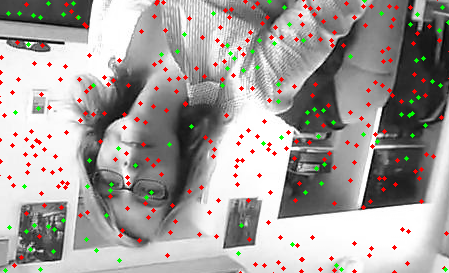
\includegraphics[scale=0.3]{./imgs/rachel_upside.png}
    \caption{
        rachel\_upside.png
    }
\end{figure}

\begin{itemize}
    \item Graphs
    \item Webcam input test
    \item Rachel flipped vs nonflipped
\end{itemize}

\end{document}
